\documentclass[11pt]{article}
\usepackage[T1]{fontenc}
\usepackage{lmodern,amsmath,amssymb,mathtools,mathrsfs,booktabs,longtable,array,microtype,graphicx}
\usepackage[a4paper,margin=24mm]{geometry}
\usepackage[hidelinks,hypertexnames=false]{hyperref}
\usepackage{xurl}
\setlength{\emergencystretch}{3em}
\providecommand{\tightlist}{\setlength{\itemsep}{0pt}\setlength{\parskip}{0pt}}
\title{Defining-prime normalization of the signed Erd\H{o}s--Straus quartic}
\author{The Clankers}
\date{20 September 2026}

\begin{document}
\maketitle
\begin{abstract}
For a positive integral Erd\H{o}s--Straus witness at a prime
$p\equiv1\pmod {12}$, this reader computes the original rank-eight signed
quartic order at its defining prime.  It gives the complete integral
normalization matrix, all Smith factors in every residue-collision stratum,
the exact translated-chart quadratic twist, two explicit $p=1201$ boundary
fibres, the fixed-prime rank-$2+6$ gluing, and the retained complex metric
minimum.  The separated exterior and middle orders have indices $p^2$ and
$p^9$.  Their normalized factors also give a typed local signed-label
representation and the conductor--index identity.  No universal occupancy,
Erd\H{o}s--Straus counterexample, zeta zero or RH conclusion is inferred.
\end{abstract}

\section*{Visual guide}
\begin{figure}[htbp]
\centering
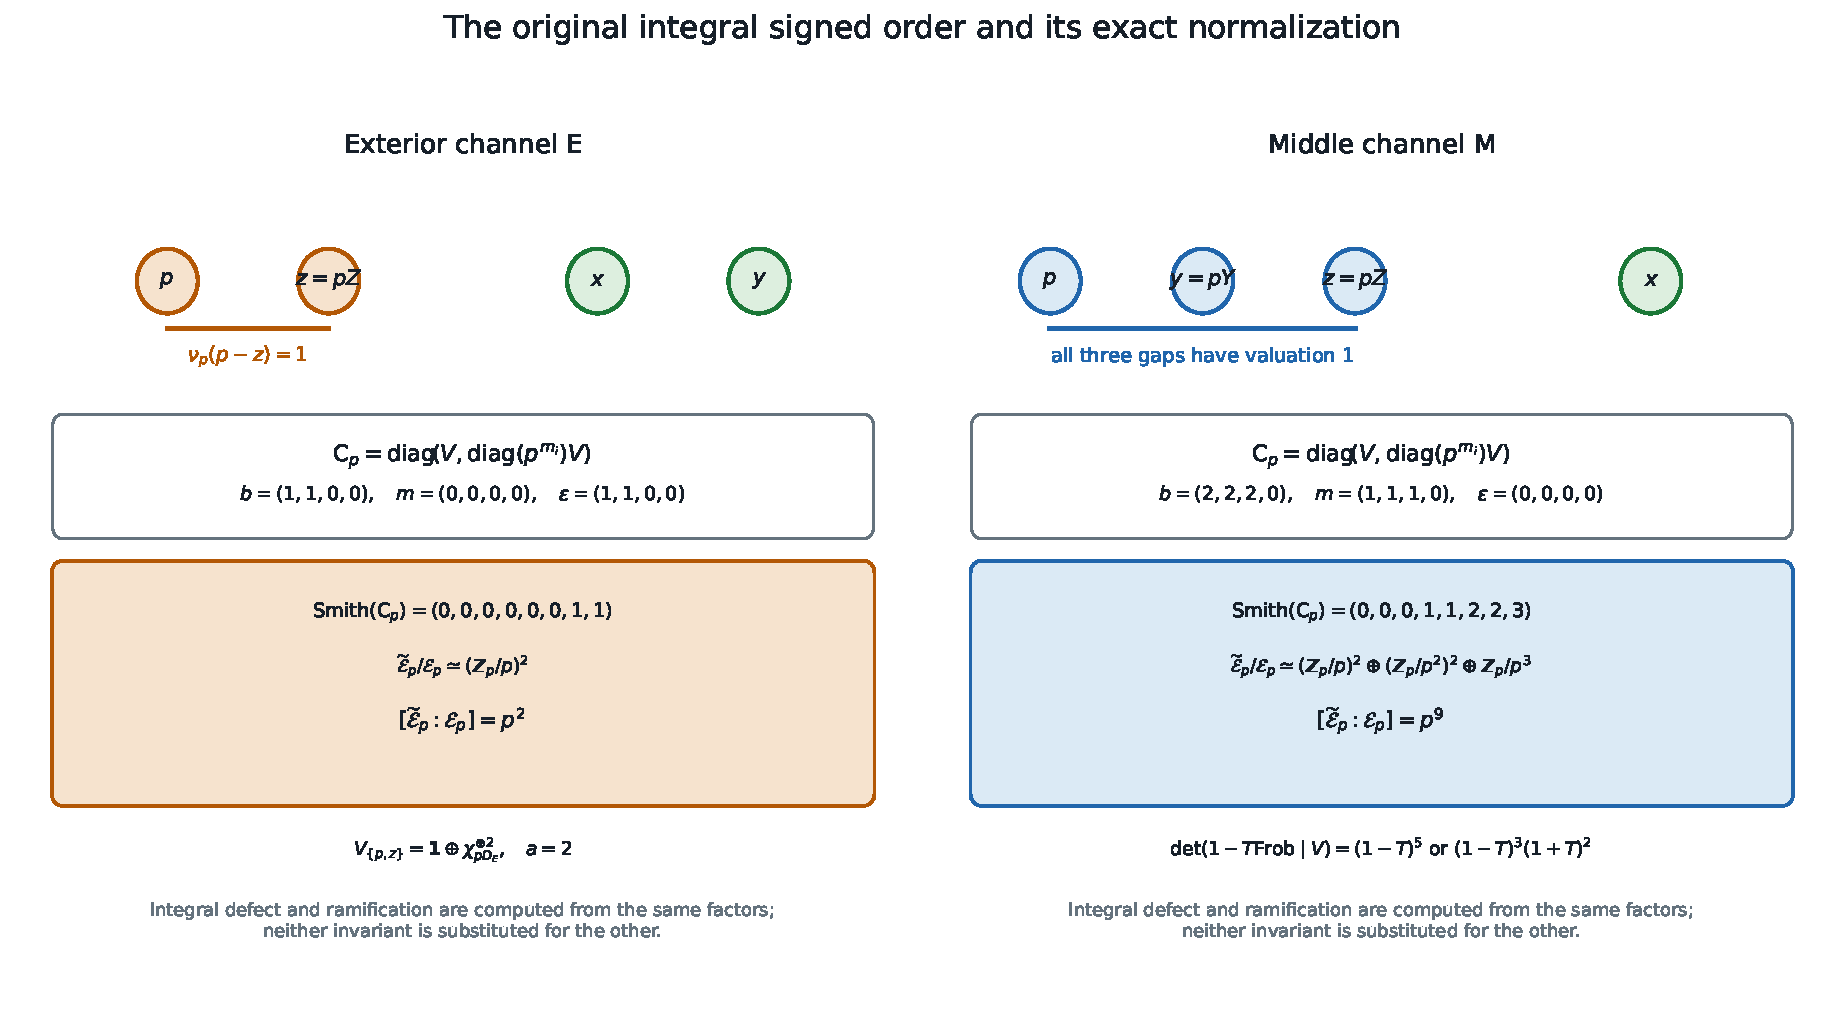
\includegraphics[width=\textwidth]{figures/integral-normalization-smith.pdf}
\caption{The exact normalization matrix specialized to the separated exterior
and middle channels.  The complete proof and identical-basis crosswalk are in
Sections~3--4 and the E/M crosswalk.}
\end{figure}

\begin{figure}[htbp]
\centering
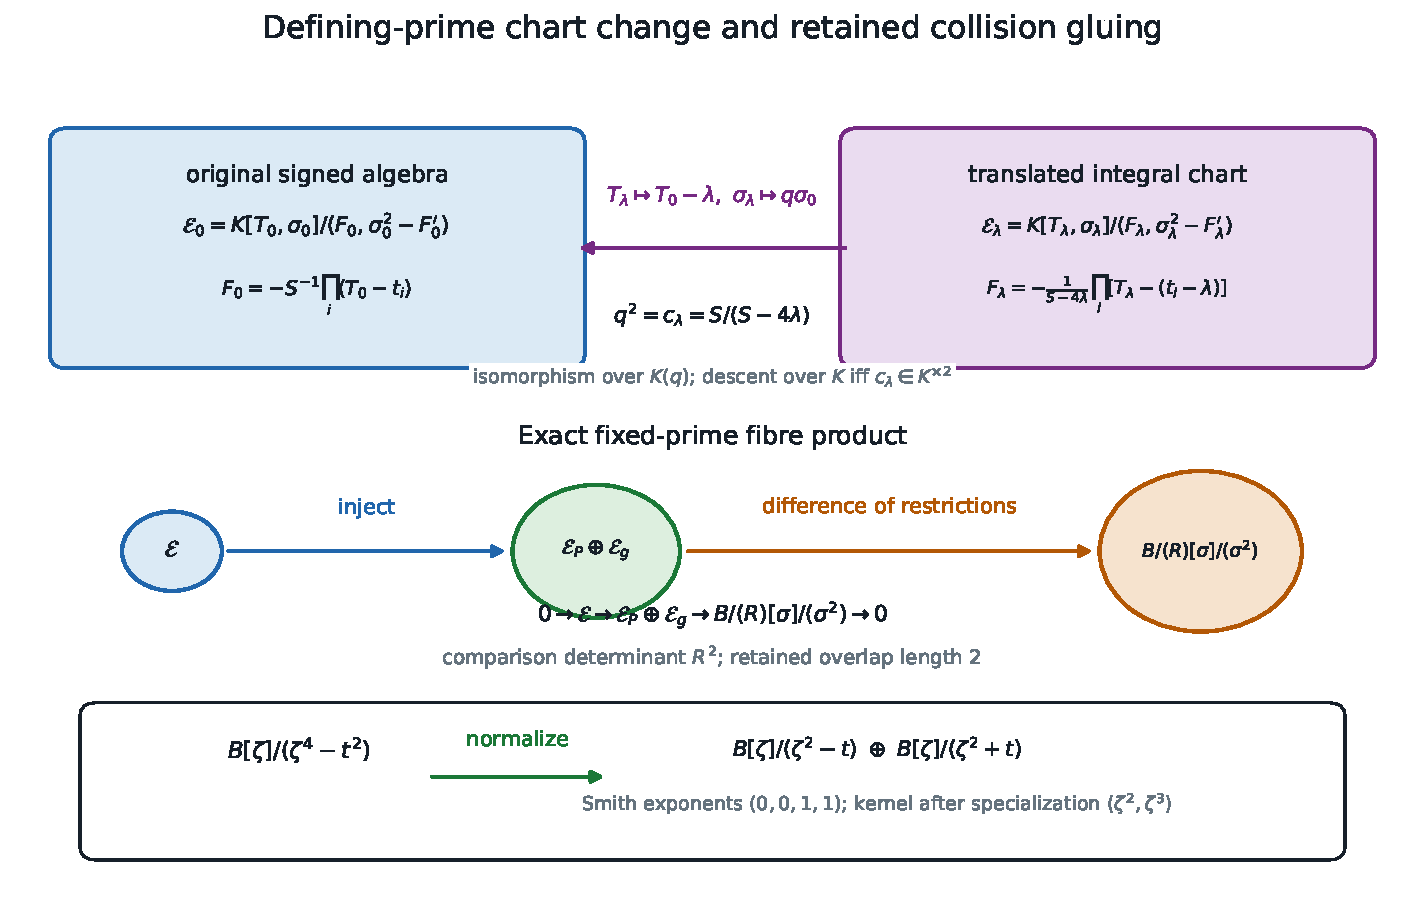
\includegraphics[width=\textwidth]{figures/defining-prime-twist-gluing.pdf}
\caption{The translated chart maps to the original signed algebra only after
the displayed quadratic base extension.  The lower row gives the exact
fixed-prime fibre product and collision normalization.}
\end{figure}

\clearpage
\section{Corrected defining-prime derivation}
\input{DEFINING_PRIME_CONTINUATION}

\clearpage
\input{INTEGRAL_NORMALIZATION_CROSSWALK}

\clearpage
\input{LOCAL_GALOIS_REPRESENTATION}
\end{document}
